% !TEX root = ../my-thesis.tex
%
\chapter{Resultados}
\label{sec:results}

Los resultados obtenidos de la implementación del problema directo y del problema inverso del EEG, así como el análisis estadístico del estimador, se presentan en tres subsecciones: (i) la solución del problema directo, (ii) la solución del problema inverso, y (iii) el análisis estadístico del error incurrido en el uso de diferentes valores del BSCR en la simulación y posterior localización de fuentes de actividad neuronal.
A su vez, debido a la gran cantidad de datos obtenidos, se presentan los de mayor relevancia en las figuras y tablas correspondientes, haciendo especial énfasis en los resultados provenientes del uso de los valores de BSCR más referidos en la literatura y los que más se alejan de estos valores, con el fin de comparar los resultados obtenidos y analizar el desempeño del estimador en cada caso.

\section{Solución del Problema Directo}
\label{sec:results:direct}


La distribución de resultados de la solución del problema directo simulando actividad neuronal con el dipolo ubicado en el área somatosensorial como fuente, se presenta en la \cref{fig:sankey-direct}, incluyendo la cantidad de pruebas realizadas por cada permutación de SNR y BSCR. 
Este mismo proceso se repitió para los dipolos ubicados en las áreas auditiva y visual, dando como resultado el total de 9000 simulaciones de señales de EEG para cada dipolo y permutación de SNR y BSCR mencionadas en la \cref{sec:methodology:direct_solved}.

\begin{figure}[tb]
    \centering
    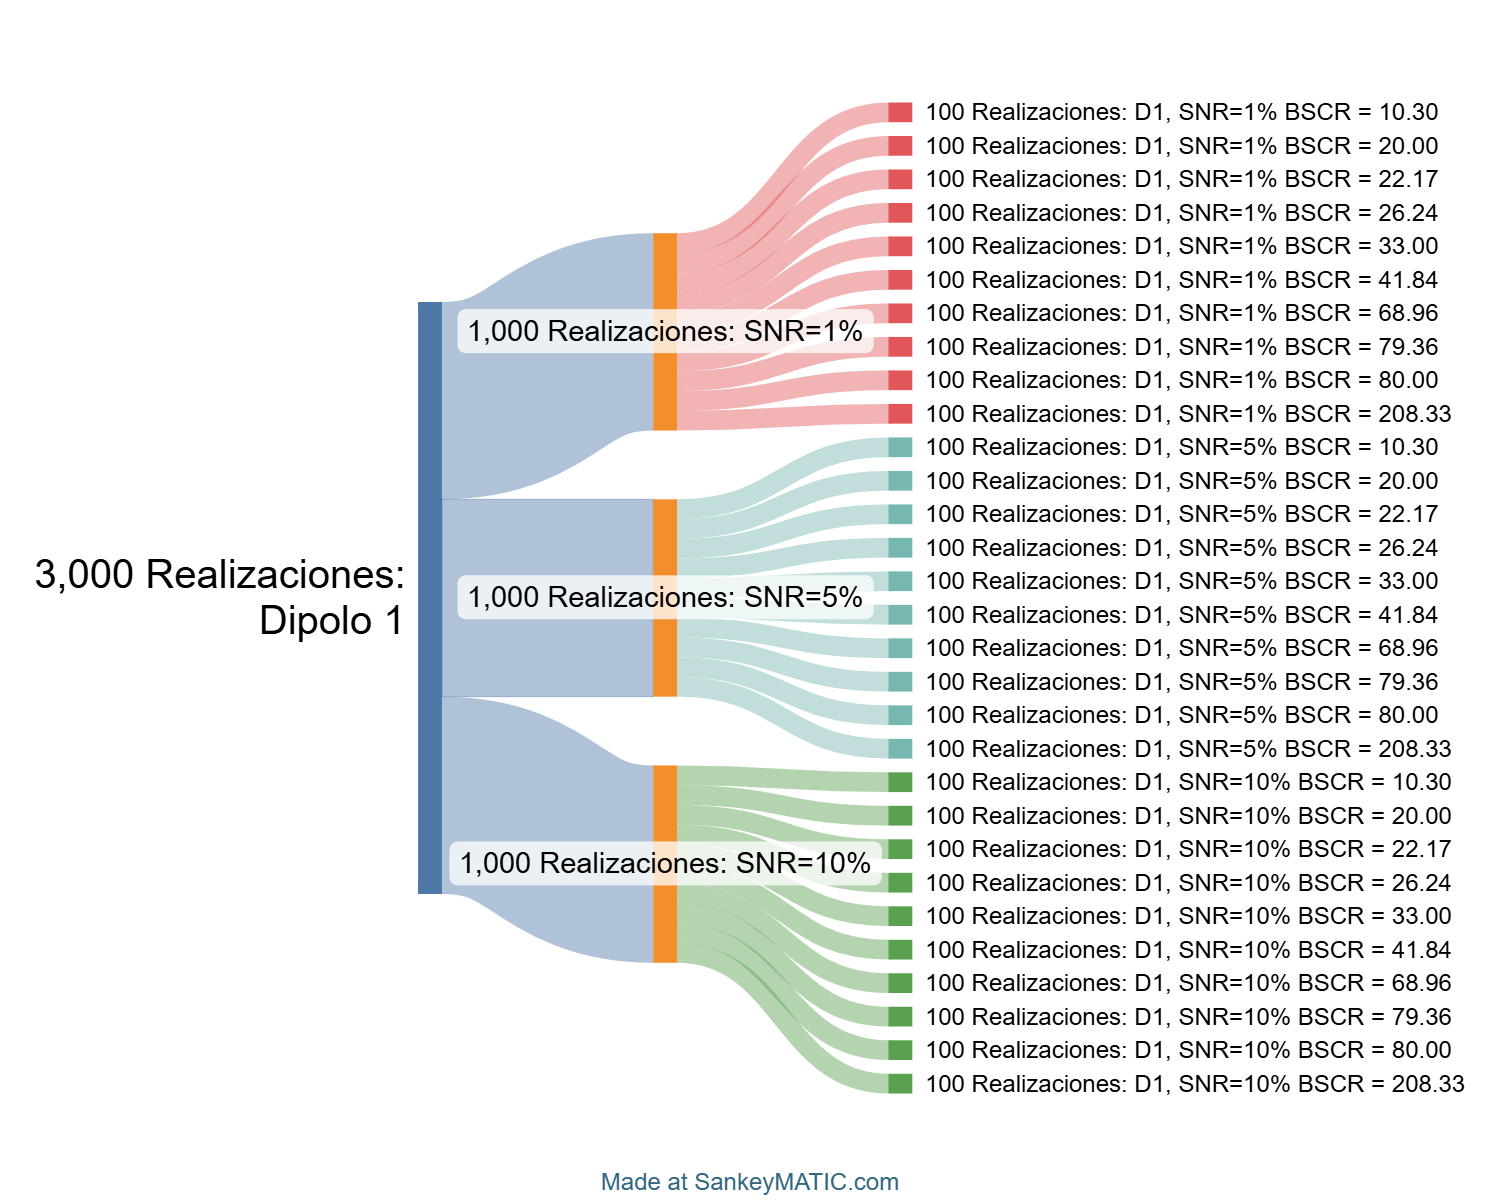
\includegraphics[width=\textwidth]{gfx/sankey-direct.png}
    \caption{Diagrama de la distribución del número de señales obtenidas en la solución del problema directo para el Dipolo 1. El mismo proceso se repitió para los Dipolos 2 y 3, dando como resultado un total de 9,000 señales simuladas.}
    \label{fig:sankey-direct}
\end{figure}

Dada la cantidad de datos obtenidos, en la \cref{fig:eeg-simulated} se presentan únicamente las señales de EEG simuladas con valores de BSCR = 10, 20, 80 y 200, con un SNR añadido de 1\%, y con origen en la zona somatosensorial. 
Esos valores de BSCR fueron seleccionados por su relevancia en la literatura (en el caso de BSCR = 20 y 80) y por ser los valores más alejados de estos (BSCR = 10 y 200).
Además, otra razón de incluir solo estas señales, es debido a que presentar los resultados individuales de todos los valores no aportaría diferencias discernibles viéndolas a este nivel de detalle (LOD, del Inglés \emph{level of detail}) y extendería el documento sin causa.

\begin{figure}[p]
    \centering
    \begin{subfigure}{\textwidth}
        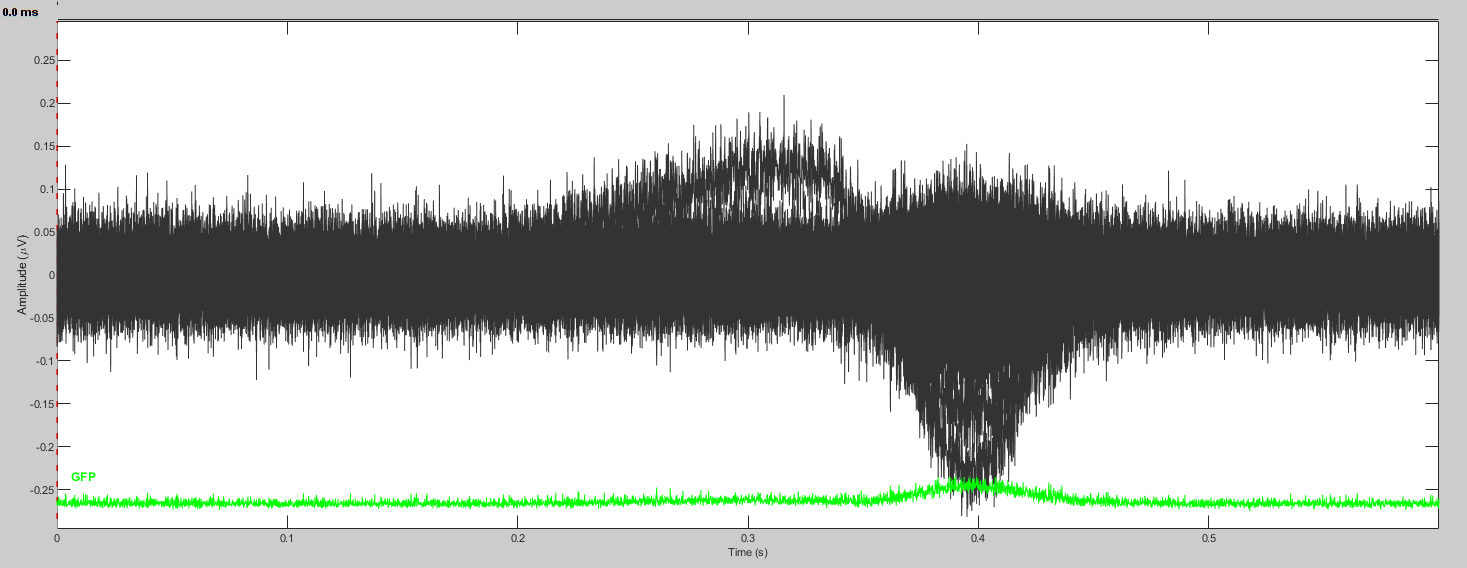
\includegraphics[height=0.23\textheight]{eeg/eeg-d1n1c8c8.png}
        \caption{Señales de EEG simuladas con BSCR = 10.}
        \label{fig:eeg-d1n1c8c8}
        \vspace{0.5em}
    \end{subfigure}
    \vfill
    \begin{subfigure}{\textwidth}
        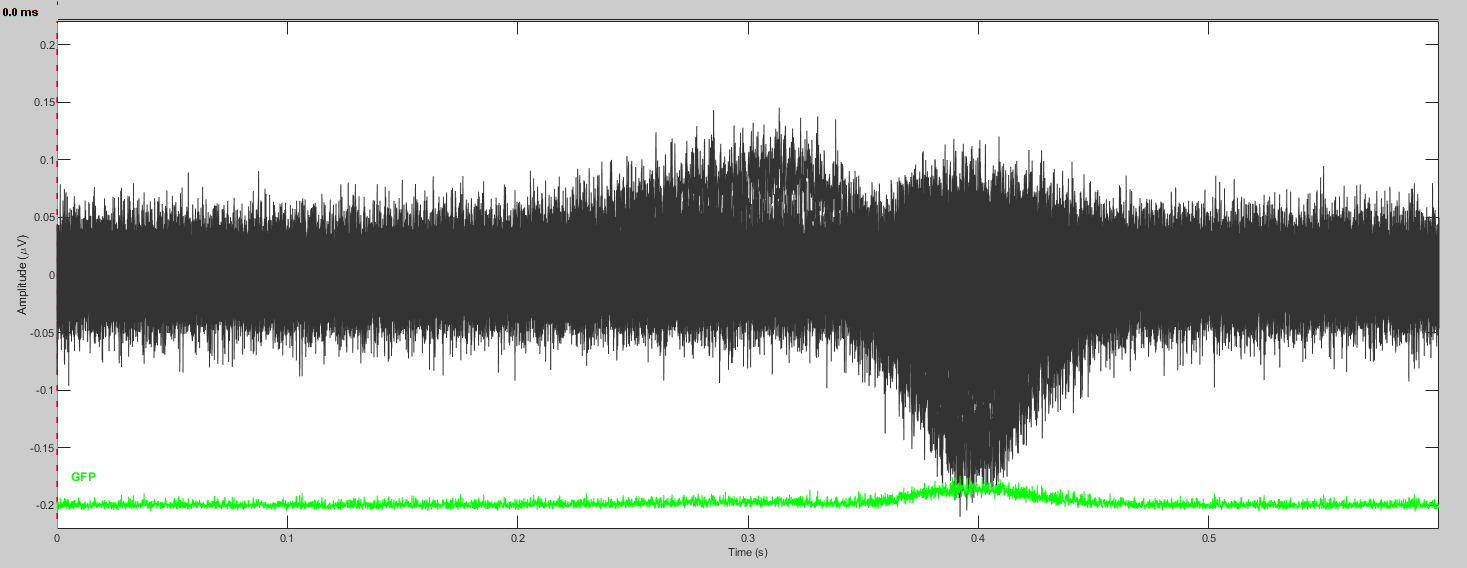
\includegraphics[height=0.23\textheight]{eeg/eeg-d1n1c9c9.png}
        \caption{Señales de EEG simuladas con BSCR = 20.}
        \label{fig:eeg-d1n1c9c9}
        \vspace{0.5em}
    \end{subfigure}
    \vfill
    \begin{subfigure}{\textwidth}
        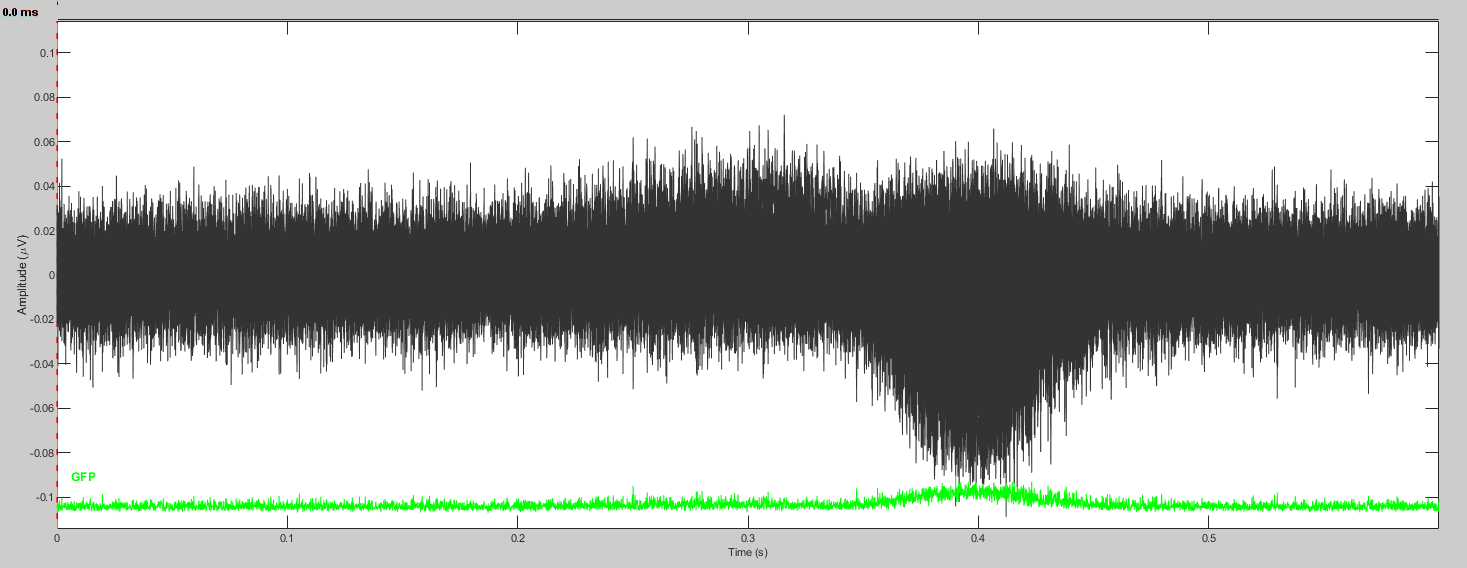
\includegraphics[height=0.23\textheight]{eeg/eeg-d1n1c10c10.png}
        \caption{Señales de EEG simuladas con BSCR = 80.}
        \label{fig:eeg-d1n1c10c10}
        \vspace{0.5em}
    \end{subfigure}
    \vfill
    \begin{subfigure}{\textwidth}
        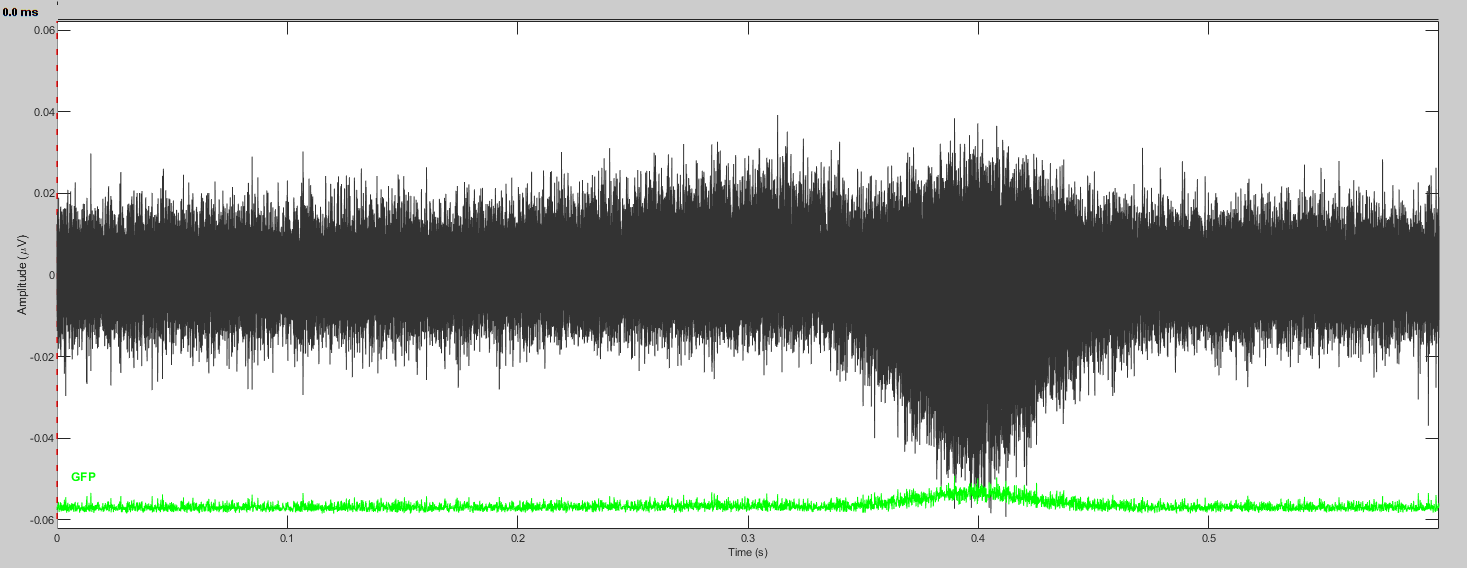
\includegraphics[height=0.23\textheight]{eeg/eeg-d1n1c2c2.png}
        \caption{Señales de EEG simuladas con BSCR = 200.}
        \label{fig:eeg-d1n1c2c2}
    \end{subfigure}
    \caption{Señales de EEG simuladas con diferentes valores de BSCR.}
    \label{fig:eeg-simulated}
\end{figure}

En cada gráfica de la \cref{fig:eeg-simulated}, se superponen las señales individuales capturadas por cada uno de los 63 electrodos considerados en el análisis, creando un gráfico de mariposa donde el eje horizontal representa el tiempo y el eje vertical representa la amplitud de la señal.
Este conjunto de señales son una parte del total de las 9000 señales simuladas por las 100 pruebas de cada permutación de BSCR, SNR y fuente de actividad neuronal.

Observando las señales simuladas, se puede apreciar que a medida que el valor de BSCR disminuye, la amplitud de las señales aumenta.
Esto no indica que la actividad neuronal sea mayor, sino que la señal es más fácil de detectar por la menor resistencia que presenta al pasar por los tejidos del cráneo.
Cabe mencionar que esta diferencia de amplitud no representa una métrica aceptable para comparar la actividad neuronal entre diferentes valores de BSCR, ya que también influyen otros factores como el ruido introducido en la simulación, el ruido generado por el equipo de medición y en casos reales, las condiciones del paciente.
Independientemente del valor de BSCR, se puede observar que las señales presentan un patrón similar, lo que indica que el estímulo simulado es el mismo en todos los casos.

\section{Solución del Problema Inverso}
\label{sec:results:inverse}

Como se mencionó en la \cref{sec:methodology:inverse_solved}, el problema inverso se resolvió variando el valor de BSCR en la implementación del filtro espacial para cada una de las 9,000 señales simuladas en el problema directo, dando como resultado un total de 90,000 mapas del PNAI.
Un ejemplo de este proceso se muestra en la \cref{fig:sankey-inverse}, donde se presenta la distribución de los resultados obtenidos en la solución del problema inverso para el dipolo ubicado en la zona somatosensorial. 
Este proceso es el contiguo al mostrado en la \cref{fig:sankey-direct} y en conjunto representan el flujo completo de la simulación y localización de fuentes de actividad neuronal en el EEG para un dipolo.

\begin{figure}[!b]
    \centering
    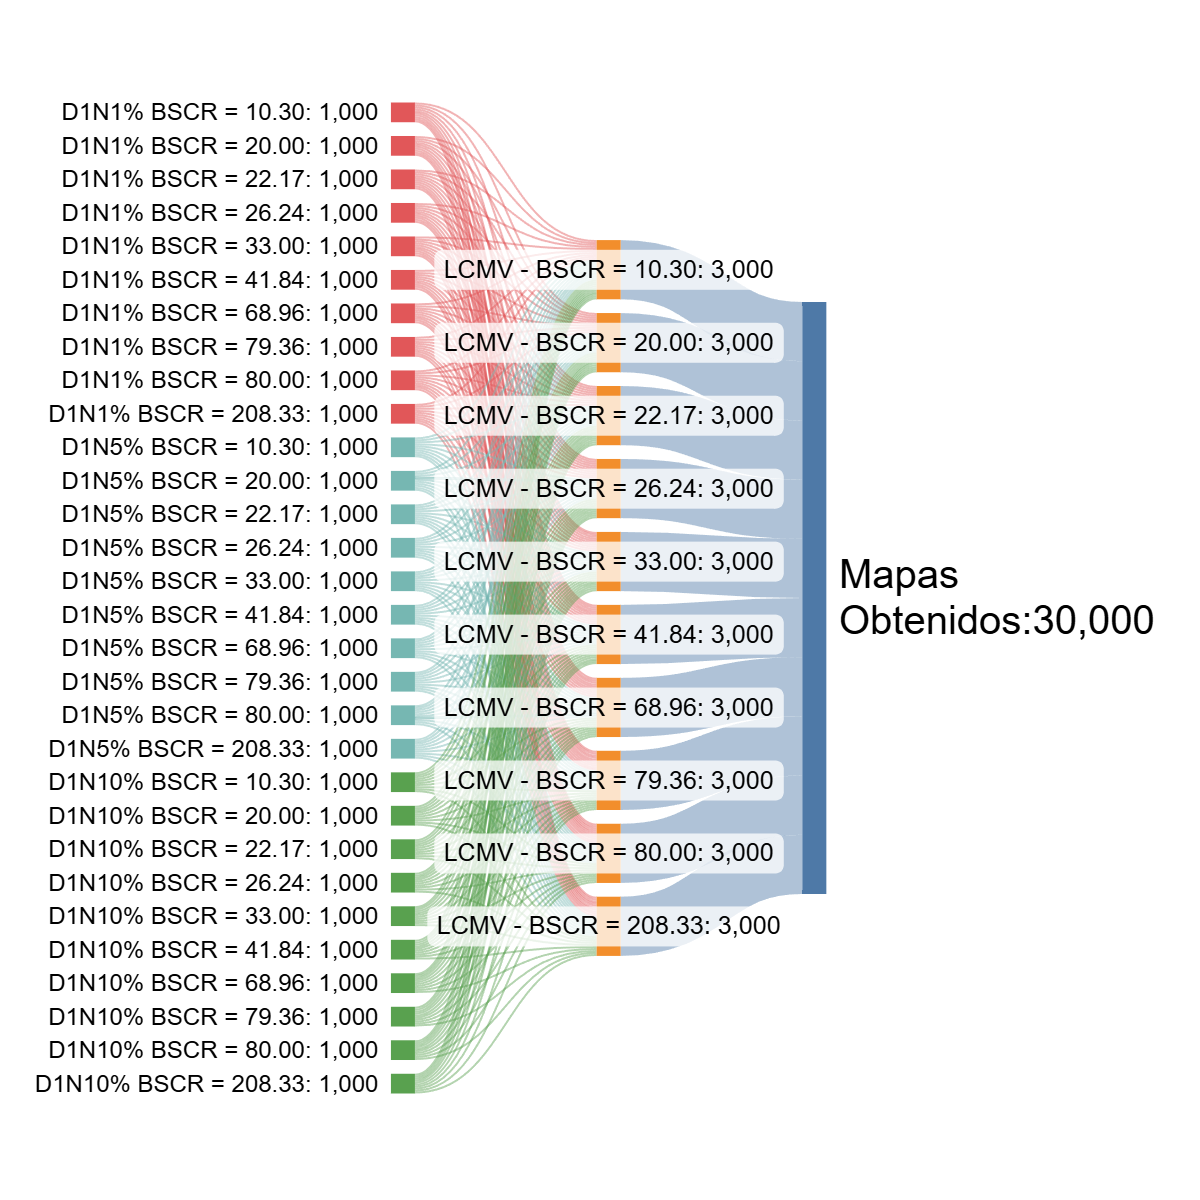
\includegraphics[width=\textwidth]{gfx/sankey-inverse.png}
    \caption{Diagrama de la distribución del número de señales obtenidas en la solución del problema directo para el dipolo 1. El mismo proceso se repitió para los dipolos 2 y 3, dando como resultado un total de 9,000 señales simuladas.}
    \label{fig:sankey-inverse}
\end{figure}

En la \cref{fig:inverse-results}, se muestran los resultados de la implementación del problema inverso para el valor de BSCR = 10, 20, 80 y 200, correspondientes al conjunto de señales simuladas con un SNR de 1\% proveniente de la fuente de actividad neuronal ubicada en la zona somatosensorial mencionadas en la \cref{sec:results:direct}.
Las señales de EEG simuladas tienen una componente en el tiempo, por tanto, el problema inverso se calcula para cada instante de tiempo correspondiente a la frecuencia de muestreo de 1000 Hz, por lo que los resultados mostrados en la \cref{fig:inverse-results} corresponden al instante de tiempo en el que la función del dipolo utilizando como fuente de actividad neuronal se encuentra en su cenit.

\begin{figure}[!b]
    \centering
    \begin{subfigure}{0.45\textwidth}
        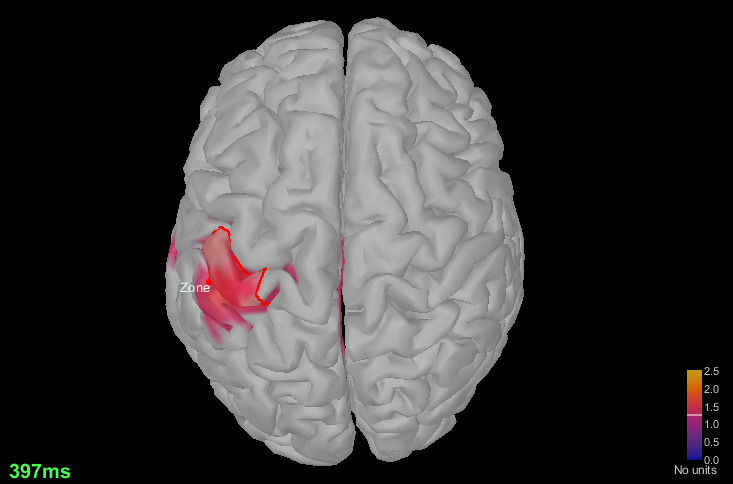
\includegraphics[width=\textwidth]{inverse/inverse-d1n1c2c2.png}
        \caption{PNAI obtenido con BSCR = 200.}
        \label{fig:inverse-d1n1c2c2}
    \end{subfigure}
    \hfill
    \begin{subfigure}{0.45\textwidth}
        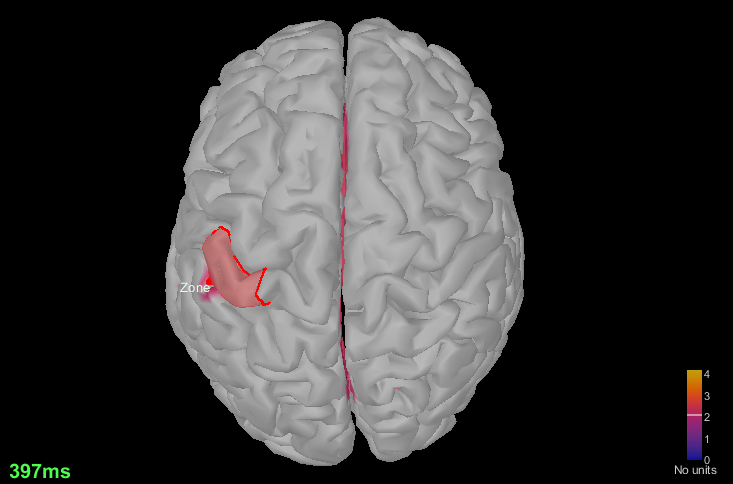
\includegraphics[width=\textwidth]{inverse/inverse-d1n1c10c10.png}
        \caption{PNAI obtenido con BSCR = 80.}
        \label{fig:inverse-d1n4c2c2}
    \end{subfigure}
    \vskip\baselineskip
    \begin{subfigure}{0.45\textwidth}
        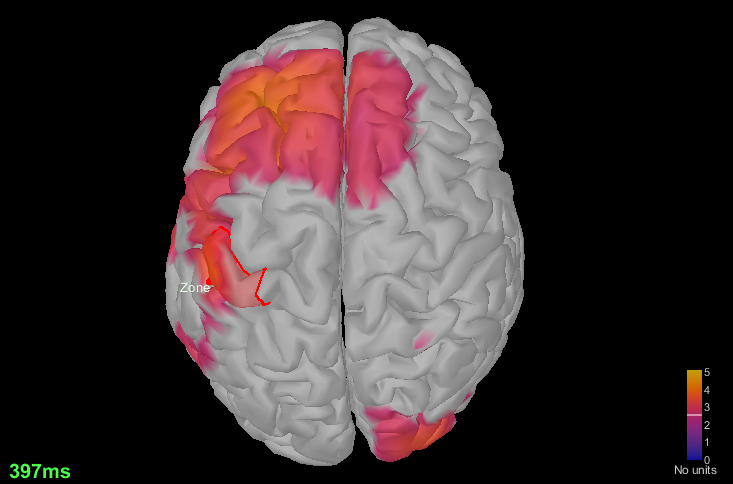
\includegraphics[width=\textwidth]{inverse/inverse-d1n1c9c9.png}
        \caption{PNAI obtenido con BSCR = 20.}
        \label{fig:inverse-d1n3c2c2}
    \end{subfigure}
    \hfill
    \begin{subfigure}{0.45\textwidth}
        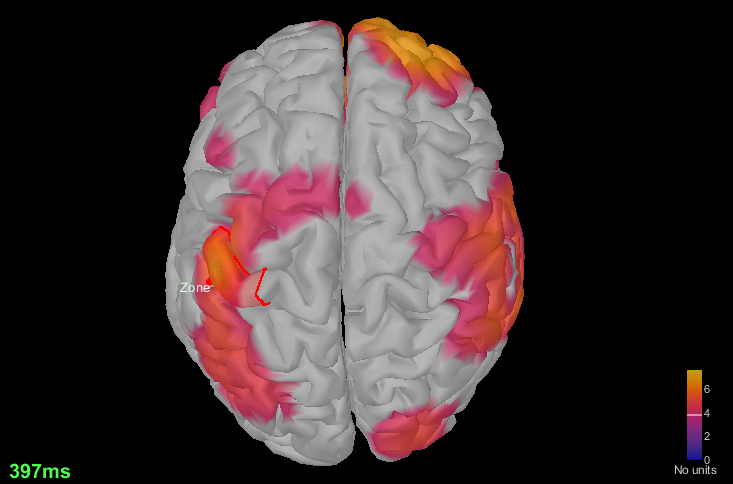
\includegraphics[width=\textwidth]{inverse/inverse-d1n1c8c8.png}
        \caption{PNAI obtenido con BSCR = 10.}
        \label{fig:inverse-d1n2c2c2}
    \end{subfigure}
    \caption{Resultados de la implementación del problema inverso con discrepancia de valores de BSCR usados en el problema directo e inverso en el dipolo ubicado en la zona somatosensorial, la cual se presenta como el área roja.}
    \label{fig:inverse-results}
    % Cambié el orden de las figuras
\end{figure}

Los resultados mostrados en la figura en cuestión, representan la proyección de la fuente de actividad neuronal en la malla representativa de la corteza cerebral en forma del mapa del PNAI.
Las mallas tienen una área marcada en rojo que corresponde a la región donde se realizó la búsqueda de las fuentes de actividad neuronal en la simulación de las señales de EEG para el dipolo ubicado en la zona somatosensorial.
Mientras que las áreas entre azul y amarillo correspondientes al rango inscrito en las figuras, representan la magnitud del PNAI, donde el azul indica la menor magnitud y el amarillo la mayor magnitud.

Las figuras muestran la localización de la fuente de actividad neuronal utilizando el mismo valor de BSCR como parámetro del filtro espacial en la solución del problema inverso y en la simulación de las señales de EEG en el problema directo.
Por lo tanto, se espera que el punto de máxima actividad neuronal proyectado sobre la malla representativa de la corteza cerebral se localice en la misma región y vértice que el dipolo utilizado como fuente de actividad neuronal en la simulación de las señales de EEG.
Justo como en los resultados de la \cref{sec:results:direct}, en la \cref{fig:inverse-results} se aprecia una diferencia en la magnitud del PNAI obtenido, donde a medida que el valor de BSCR disminuye, no solo la magnitud del PNAI aumenta, sino que también el área sobre la que se propaga la actividad neuronal simulada se expande.

\section{Error en la Localización de la Fuente de Actividad Neuronal}
\label{sec:results:error}

La estimación del error en la localización se obtuvo con el método descrito en la \cref{sec:methodology:estimator}, mientras que el análisis estadístico del desempeño del estimador se realizó con el método descrito en la \cref{sec:methodology:cbr-analysis}.
Por lo tanto, los resultados presentados en esta sección, corresponden a la diferencia entre la localización de la fuente de actividad neuronal obtenida en el problema inverso y la localización de la fuente de actividad neuronal utilizada en la simulación de las señales de EEG en el problema directo, dividida por la distancia media entre los vértices de la malla representativa de la corteza cerebral.

Con el fin de analizar y representar de manera gráfica los resultados obtenidos, se agruparon los valores del error en la localización de la fuente de actividad neuronal obtenidos en las 100 pruebas de cada permutación de BSCR, SNR y fuente de actividad neuronal, por cada implementación del filtro espacial (LCMV) en el problema inverso. 
La \cref{fig:individual-lod} ejemplifica visualmente la distribución de los valores del error para una de las permutaciones de la solución del problema directo, específicamente el caso del dipolo ubicado en la zona somatosensorial, con un SNR = 1\%, y un valor de BSCR = 20 en la solución del problema directo (D1, SNR=1\% BSCR = 20.00).

\begin{figure}[t]
    \centering
    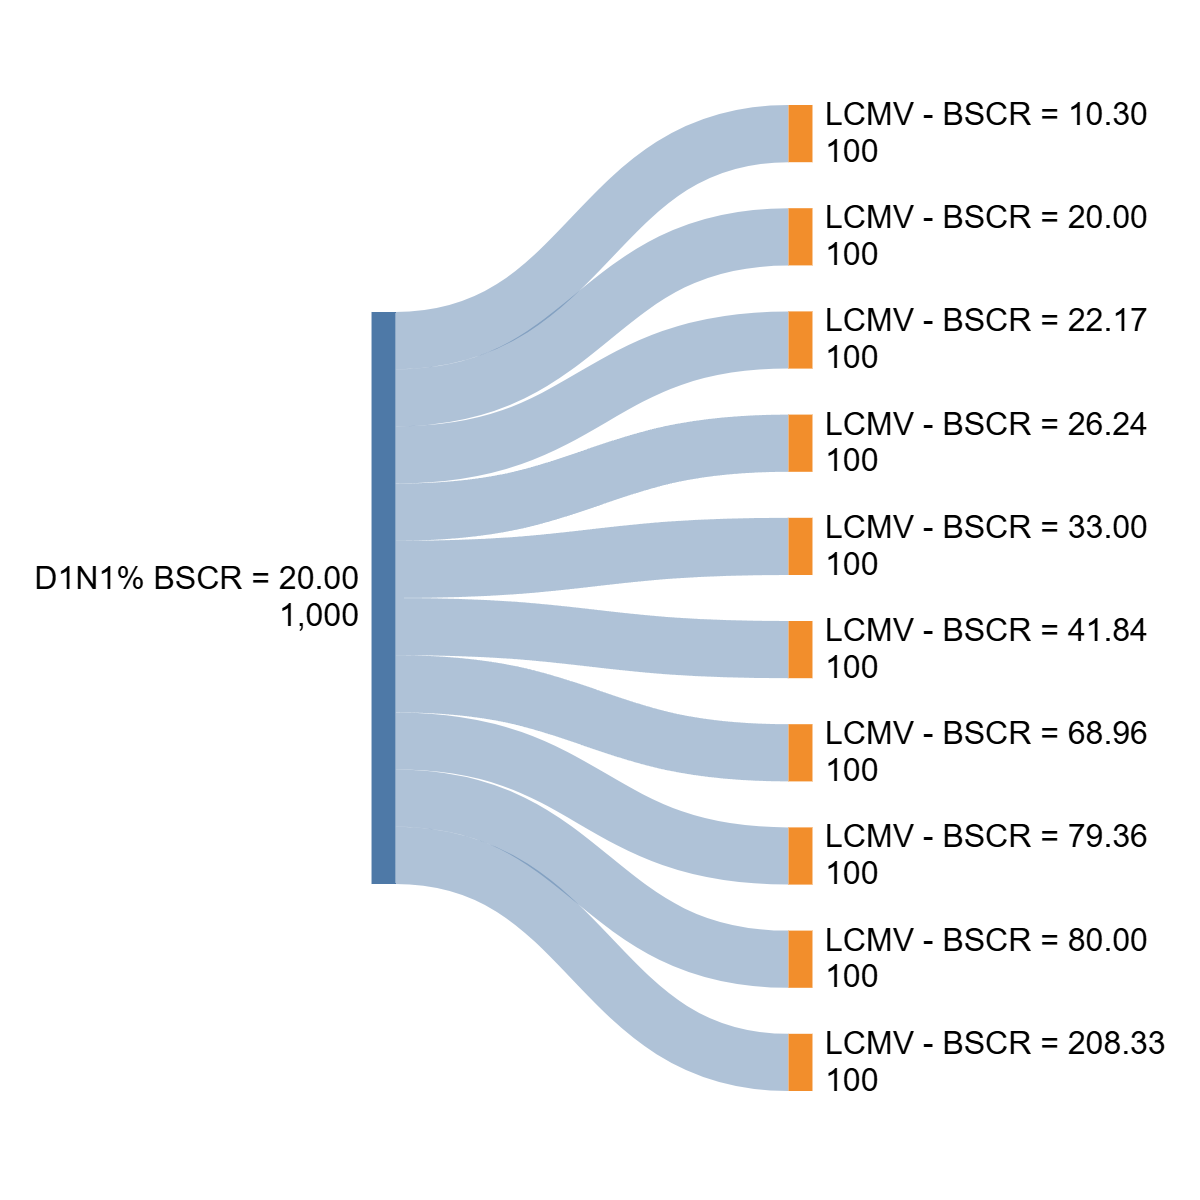
\includegraphics[width=0.9\textwidth]{gfx/individual_lod.png}
    \caption{Distribución de los valores del error en la localización de la fuente de actividad neuronal obtenidos del filtro espacial. Cada grupo es una solución con un valor distinto de BSCR de las 100 pruebas de la permutación D1, SNR=1\% BSCR = 20.00, dando como resultado 1,000 valores del error.}
    \label{fig:individual-lod}
\end{figure}

En la \cref{fig:error-results-d1n1} se muestran los resultados obtenidos en la estimación del error en la localización de la fuente de actividad neuronal con el dipolo ubicado en la zona somatosensorial (Dipolo 1 de acuerdo a nuestro sistema de identificación) y un SNR = 1\%.
Las gráficas representan el error en la localización de la fuente de actividad neuronal para los valores de BSCR = 10, 20, 80 y 200.
Estas gráficas siguen la misma estructura descrita anteriormente en la agrupación de sus datos, siendo la \cref{fig:error-d1c9n1} la correspondiente a la permutación D1, SNR=1\% BSCR = 20.00 de la \cref{fig:individual-lod}.

\begin{figure}[t]
    \centering
    \begin{subfigure}{0.49\textwidth}
        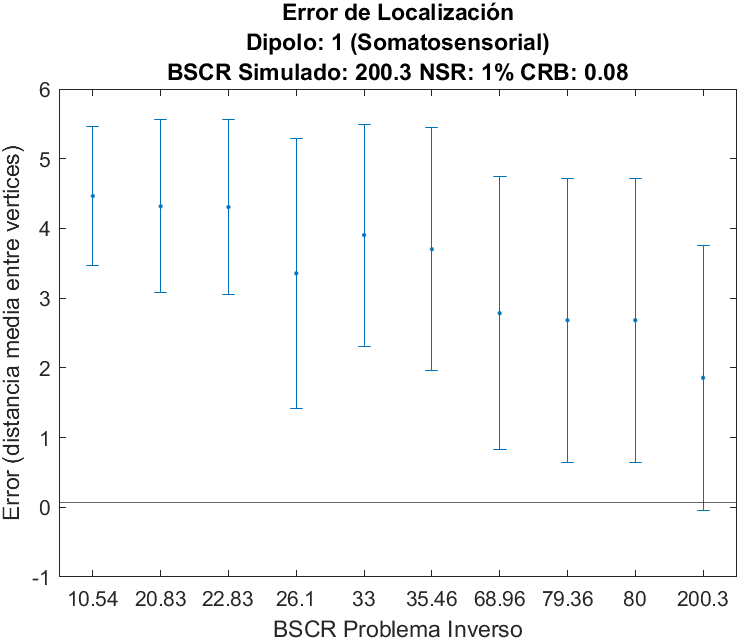
\includegraphics[width=\textwidth]{individual_graphs/d1c2n1.png}
        \caption{Error en la localización de la fuente de actividad neuronal con BSCR 200.}
        \label{fig:error-d1c2n1}
    \end{subfigure}
    \hfill
    \begin{subfigure}{0.49\textwidth}
        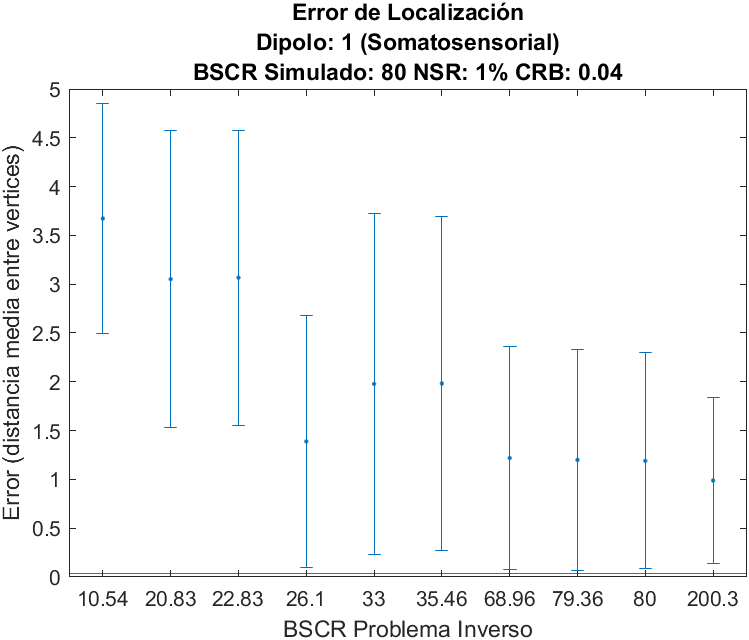
\includegraphics[width=\textwidth]{individual_graphs/d1c10n1.png}
        \caption{Error en la localización de la fuente de actividad neuronal con BSCR 80.}
        \label{fig:error-d1c10n1}
    \end{subfigure}
    \vskip\baselineskip
    \begin{subfigure}{0.49\textwidth}
        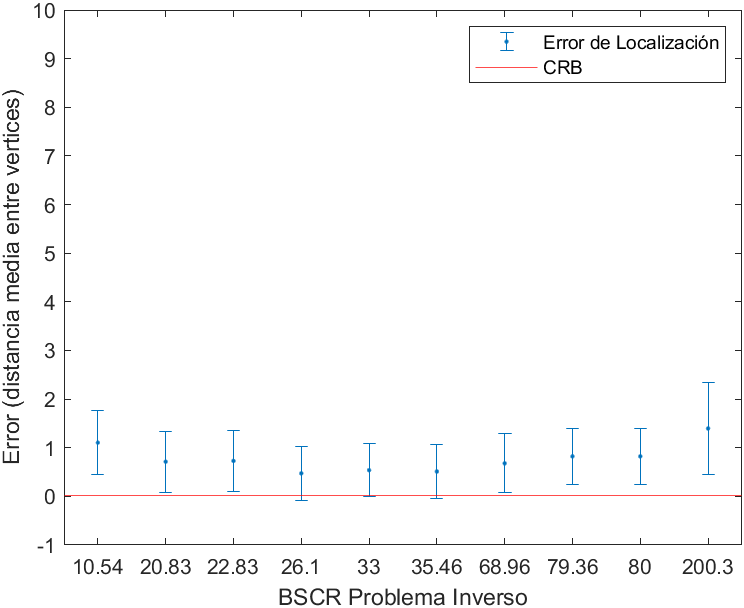
\includegraphics[width=\textwidth]{individual_graphs/d1c9n1.png}
        \caption{Error en la localización de la fuente de actividad neuronal con BSCR 20.}
        \label{fig:error-d1c9n1}
    \end{subfigure}
    \hfill
    \begin{subfigure}{0.49\textwidth}
        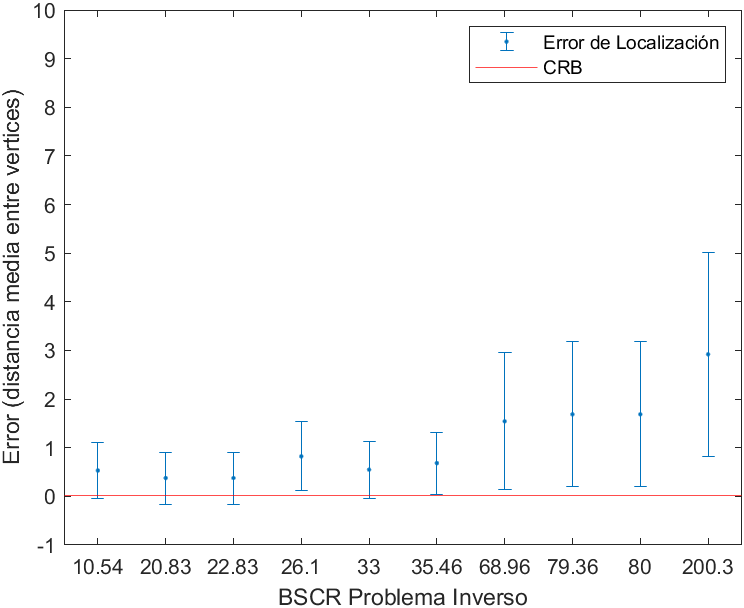
\includegraphics[width=\textwidth]{individual_graphs/d1c8n1.png}
        \caption{Error en la localización de la fuente de actividad neuronal con BSCR 10.}
        \label{fig:error-d1c8n1}
    \end{subfigure}
    \caption{Error incurrido en la localización de la fuente de actividad neuronal en con el dipolo en la zona somatosensorial y SNR = 1\%.}
    \label{fig:error-results-d1n1}
    % Cambié el orden de las figuras y el límite del eje y
\end{figure}

En cada gráfica, el eje horizontal muestra los valores de BSCR utilizados en la solución del problema inverso, mientras que el eje vertical indica la media del error la localización de la fuente de actividad neuronal obtenido en las 100 pruebas de cada permutación de BSCR en función de la distancia media entre vértices de la malla de la corteza cerebral.
Las barras de error representan la desviación estándar de los valores del error obtenidos en cada permutación, también en función de la distancia media entre vértices de la malla de la corteza cerebral. 
Por último, la línea horizontal perpendicular a las barras de error representa la CRB calculada para el estimador en cada caso, la cual indica el error mínimo que se puede obtener con un estimador no sesgado.

Tomando en cuenta la cantidad de resultados obtenidos, la atipicidad de los valores de BSCR = 10 y 200, y poca variabilidad en los resultados obtenidos con BSCRs cercanos entre sí, se enfocó el análisis en los valores de BSCR = 20 y 80 con el fin de ampliar el panorama de los datos obtenidos.
La razón de esto, es que los valores de BSCR = 20 y 80 son los más cercanos a los reportados en la literatura y que siguen presentando una diferencia significativa en la conductividad de los tejidos del cráneo.
Esta reducción en los datos disponibles nos ofrece una perspectiva más realista de los resultados obtenidos en la simulación y localización de fuentes de actividad neuronal en el EEG, al permitirnos presentar resultados más claros, concisos y relevantes para el análisis de los datos.

Específicamente, se presentan los resultados obtenidos de la solución del problema inverso de las señales de EEG simuladas con el dipolo ubicado en las zonas auditiva (Dipolo 2) y visual (Dipolo 3) y con niveles de SNR = 1\%, 5\% y 10\% para los valores de BSCR = 20 y 80.
En la \cref{fig:error-results-d2} se presentan los resultados obtenidos con el dipolo ubicado en el área auditiva, mientras que en la \cref{fig:error-results-d3} se presentan los resultados obtenidos con el dipolo ubicado en el área visual.
Las gráficas de ambas figuras siguen la misma estructura ya descrita de la \cref{fig:error-results-d1n1}, con la distribución de los valores del error en la localización de la fuente de actividad neuronal en la forma de la \cref{fig:individual-lod}.

\begin{figure}[p]
    \centering
    \begin{subfigure}{0.49\textwidth}
        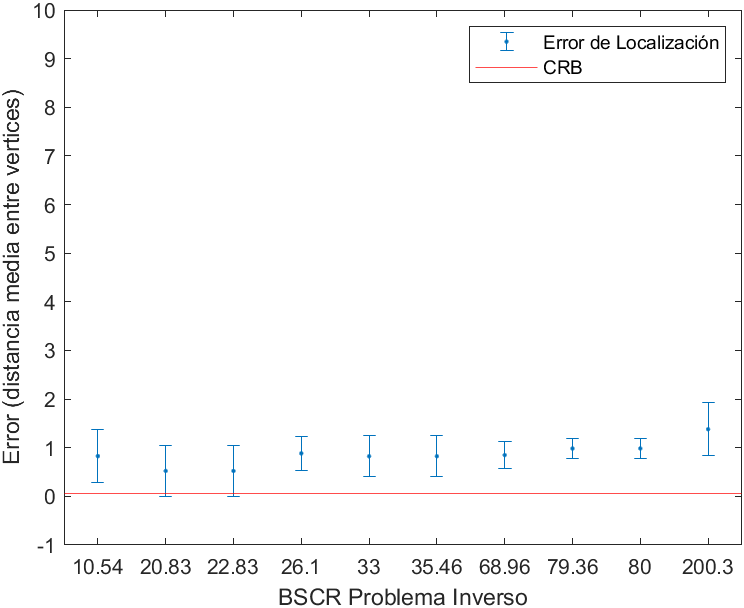
\includegraphics[width=\textwidth]{individual_graphs/d2c9n1.png}
        \caption{Error en la localización de la fuente de actividad neuronal con BSCR = 20 y SNR = 1\%.}
        \label{fig:error-d2c9n1}
    \end{subfigure}
    \hfill
    \begin{subfigure}{0.49\textwidth}
        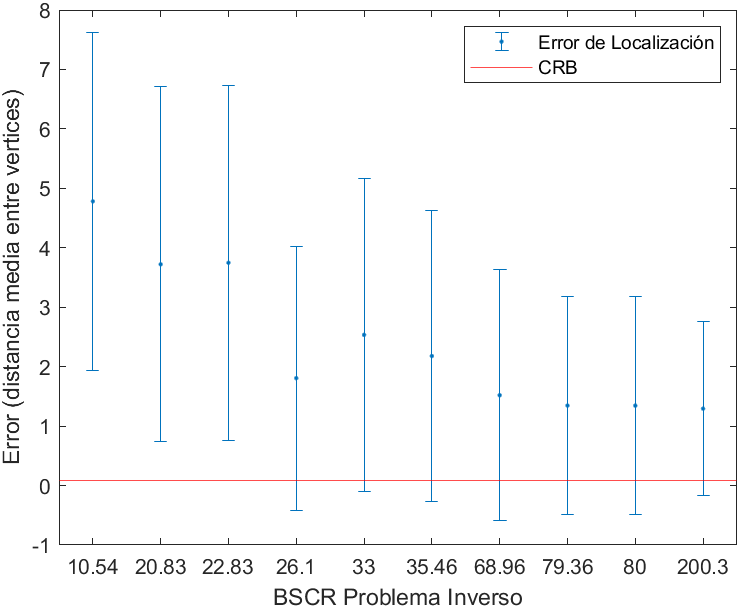
\includegraphics[width=\textwidth]{individual_graphs/d2c10n1.png}
        \caption{Error en la localización de la fuente de actividad neuronal con BSCR = 80 y SNR = 1\%.}
        \label{fig:error-d2c10n1}
    \end{subfigure}
    \vskip\baselineskip
    \begin{subfigure}{0.49\textwidth}
        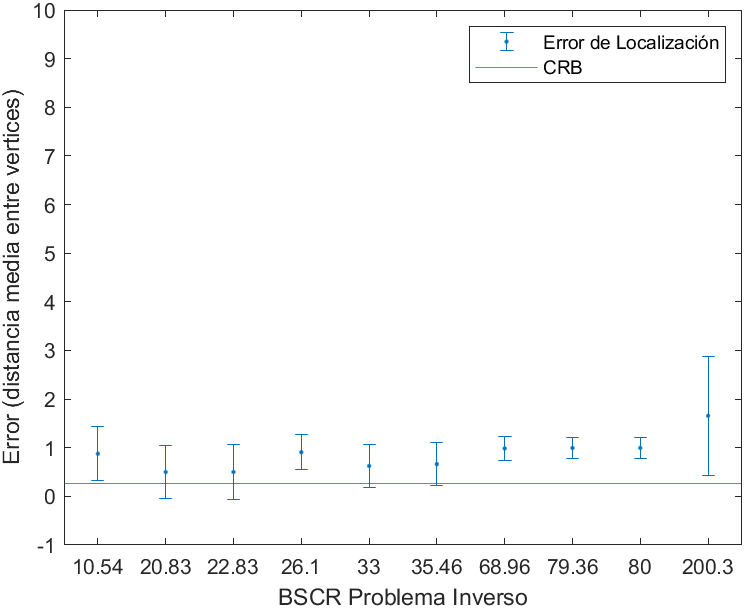
\includegraphics[width=\textwidth]{individual_graphs/d2c9n2.png}
        \caption{Error en la localización de la fuente de actividad neuronal con BSCR = 20 SNR = 5\%.}
        \label{fig:error-d2c9n2}
    \end{subfigure}
    \hfill
    \begin{subfigure}{0.49\textwidth}
        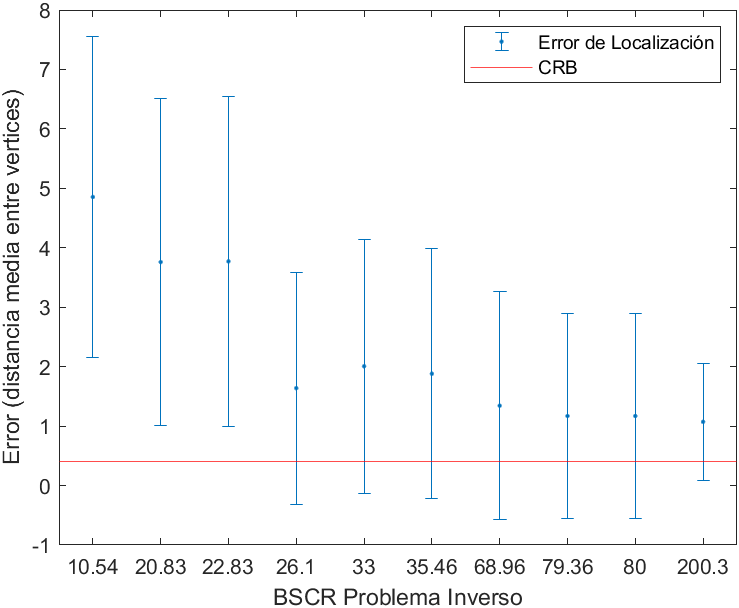
\includegraphics[width=\textwidth]{individual_graphs/d2c10n2.png}
        \caption{Error en la localización de la fuente de actividad neuronal con BSCR = 80 y SNR = 5\%.}
        \label{fig:error-d2c10n2}
    \end{subfigure}
    \vskip\baselineskip
    \begin{subfigure}{0.49\textwidth}
        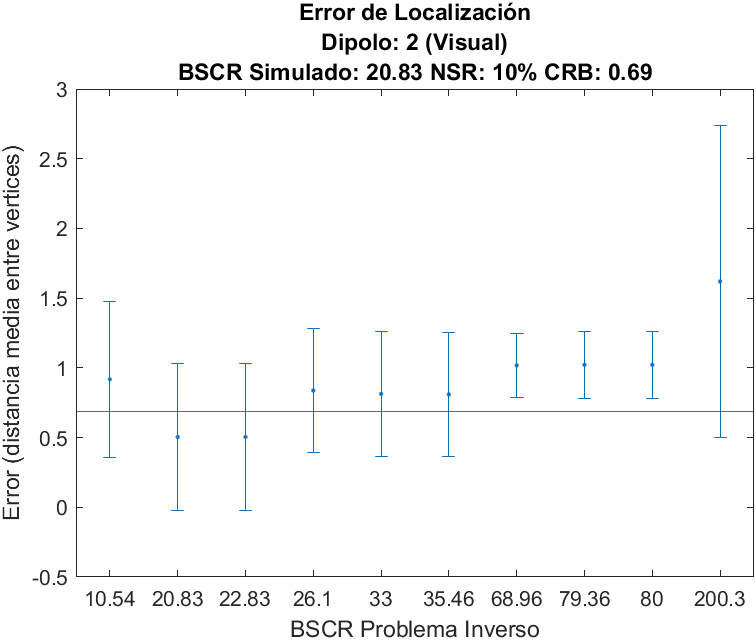
\includegraphics[width=\textwidth]{individual_graphs/d2c9n3.png}
        \caption{Error en la localización de la fuente de actividad neuronal con BSCR = 20 y SNR = 10\%.}
        \label{fig:error-d2c9n3}
    \end{subfigure}
    \hfill
    \begin{subfigure}{0.49\textwidth}
        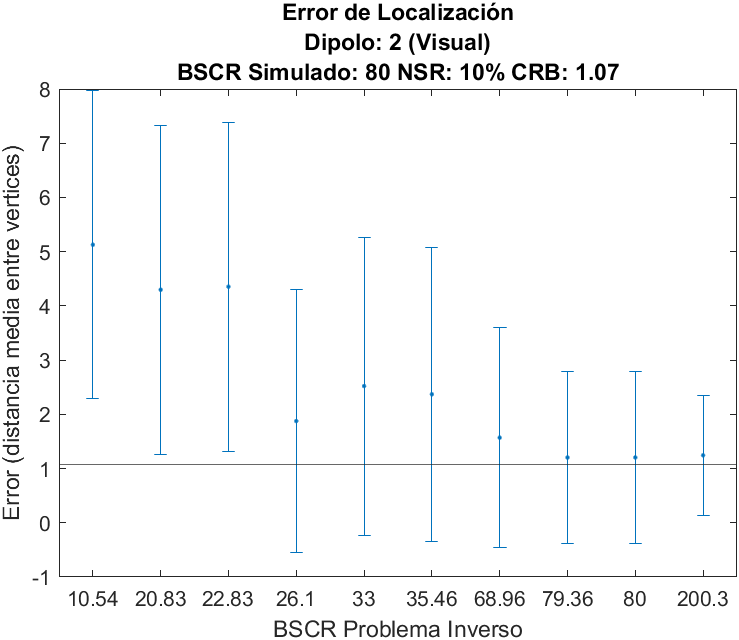
\includegraphics[width=\textwidth]{individual_graphs/d2c10n3.png}
        \caption{Error en la localización de la fuente de actividad neuronal con BSCR = 80 y SNR = 10\%.}
        \label{fig:error-d2c10n3}
    \end{subfigure}
    \caption{Error incurrido en la localización de la fuente de actividad neuronal en con el dipolo en la zona auditiva y los tres niveles de SNR.}
    \label{fig:error-results-d2}
\end{figure}

\begin{figure}[p]
    \centering
    \begin{subfigure}{0.49\textwidth}
        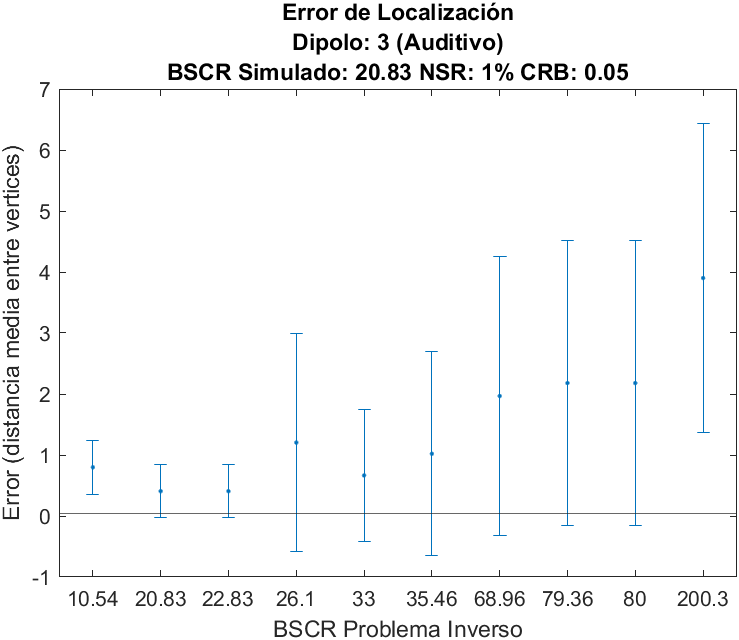
\includegraphics[width=\textwidth]{individual_graphs/d3c9n1.png}
        \caption{Error en la localización de la fuente de actividad neuronal con BSCR = 20 y SNR = 1\%.}
        \label{fig:error-d3c9n1}
    \end{subfigure}
    \hfill
    \begin{subfigure}{0.49\textwidth}
        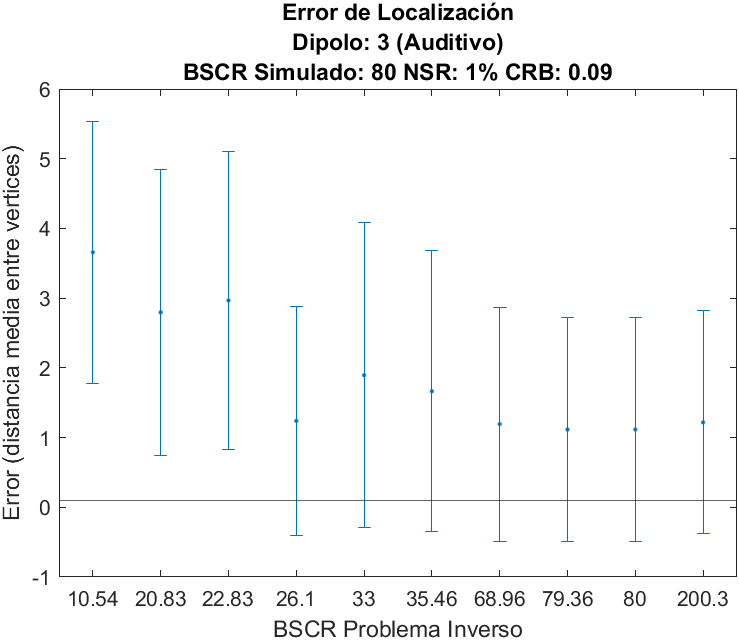
\includegraphics[width=\textwidth]{individual_graphs/d3c10n1.png}
        \caption{Error en la localización de la fuente de actividad neuronal con BSCR = 80 y SNR = 1\%.}
        \label{fig:error-d3c10n1}
    \end{subfigure}
    \vskip\baselineskip
    \begin{subfigure}{0.49\textwidth}
        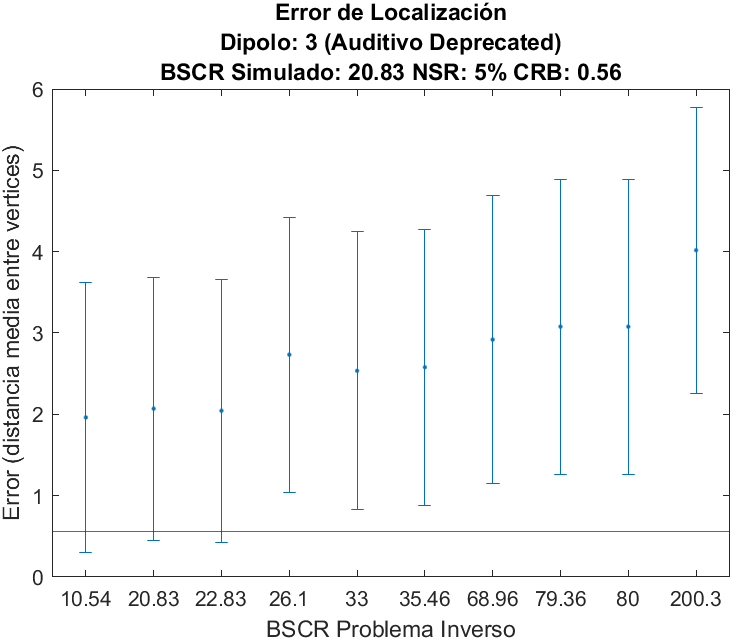
\includegraphics[width=\textwidth]{individual_graphs/d3c9n2.png}
        \caption{Error en la localización de la fuente de actividad neuronal con BSCR = 20 SNR = 5\%.}
        \label{fig:error-d3c9n2}
    \end{subfigure}
    \hfill
    \begin{subfigure}{0.49\textwidth}
        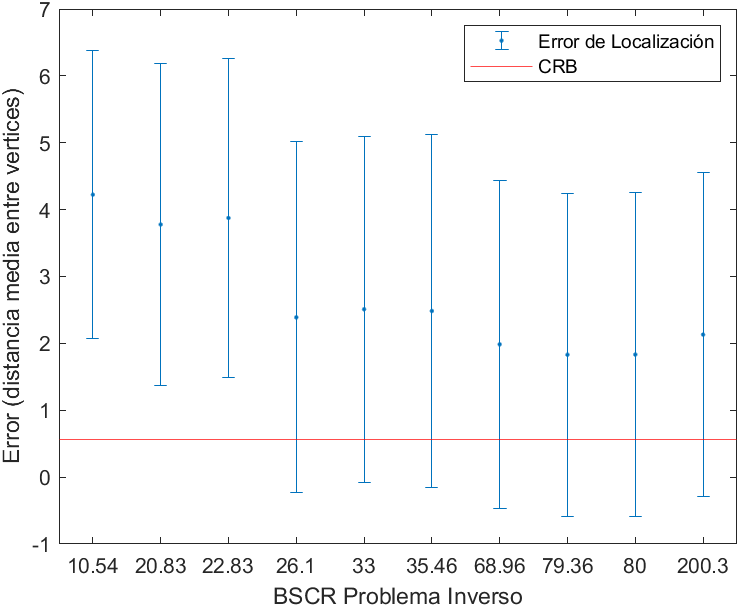
\includegraphics[width=\textwidth]{individual_graphs/d3c10n2.png}
        \caption{Error en la localización de la fuente de actividad neuronal con BSCR = 80 y SNR = 5\%.}
        \label{fig:error-d3c10n2}
    \end{subfigure}
    \vskip\baselineskip
    \begin{subfigure}{0.49\textwidth}
        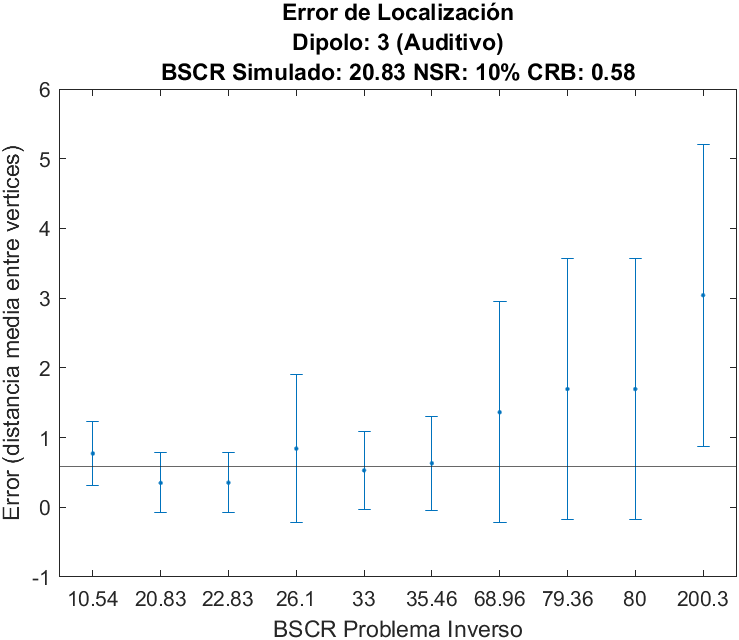
\includegraphics[width=\textwidth]{individual_graphs/d3c9n3.png}
        \caption{Error en la localización de la fuente de actividad neuronal con BSCR = 20 y SNR = 10\%.}
        \label{fig:error-d3c9n3}
    \end{subfigure}
    \hfill
    \begin{subfigure}{0.49\textwidth}
        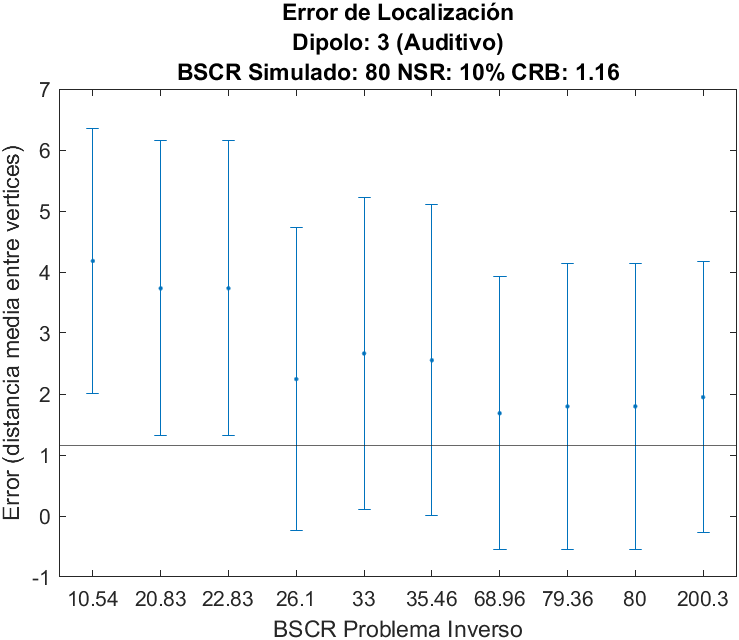
\includegraphics[width=\textwidth]{individual_graphs/d3c10n3.png}
        \caption{Error en la localización de la fuente de actividad neuronal con BSCR = 80 y SNR = 10\%.}
        \label{fig:error-d3c10n3}
    \end{subfigure}
    \caption{Error incurrido en la localización de la fuente de actividad neuronal en con el dipolo en la zona auditiva y los tres niveles de SNR.}
    \label{fig:error-results-d3}
\end{figure}

%\newpage

\section{Evaluación del Error Incurrido en la Localización de Fuentes de Actividad Neuronal}
\label{sec:results:bscr-performance}

Buscando analizar nuestros resultados en un contexto más amplio, se precedió a agrupar los resultados de más valores de BSCR y SNR en un LOD más general.
Esto se realizó agrupando todos los resultados obtenidos en la estimación del error en la localización de la fuente de actividad neuronal para cada uno de los BSCR involucrados en el problema directo, agrupados por el dipolo y nivel de ruido correspondiente, sin considerar diferencias en los valores de BSCR utilizados en el cálculo del filtro espacial en el problema inverso.
Un diagrama de este agrupamiento se presenta en la \cref{fig:sankey-boxplots}, donde se muestra el caso del dipolo 1 con un SNR = 1\%.

\begin{figure}[t]
    \centering
    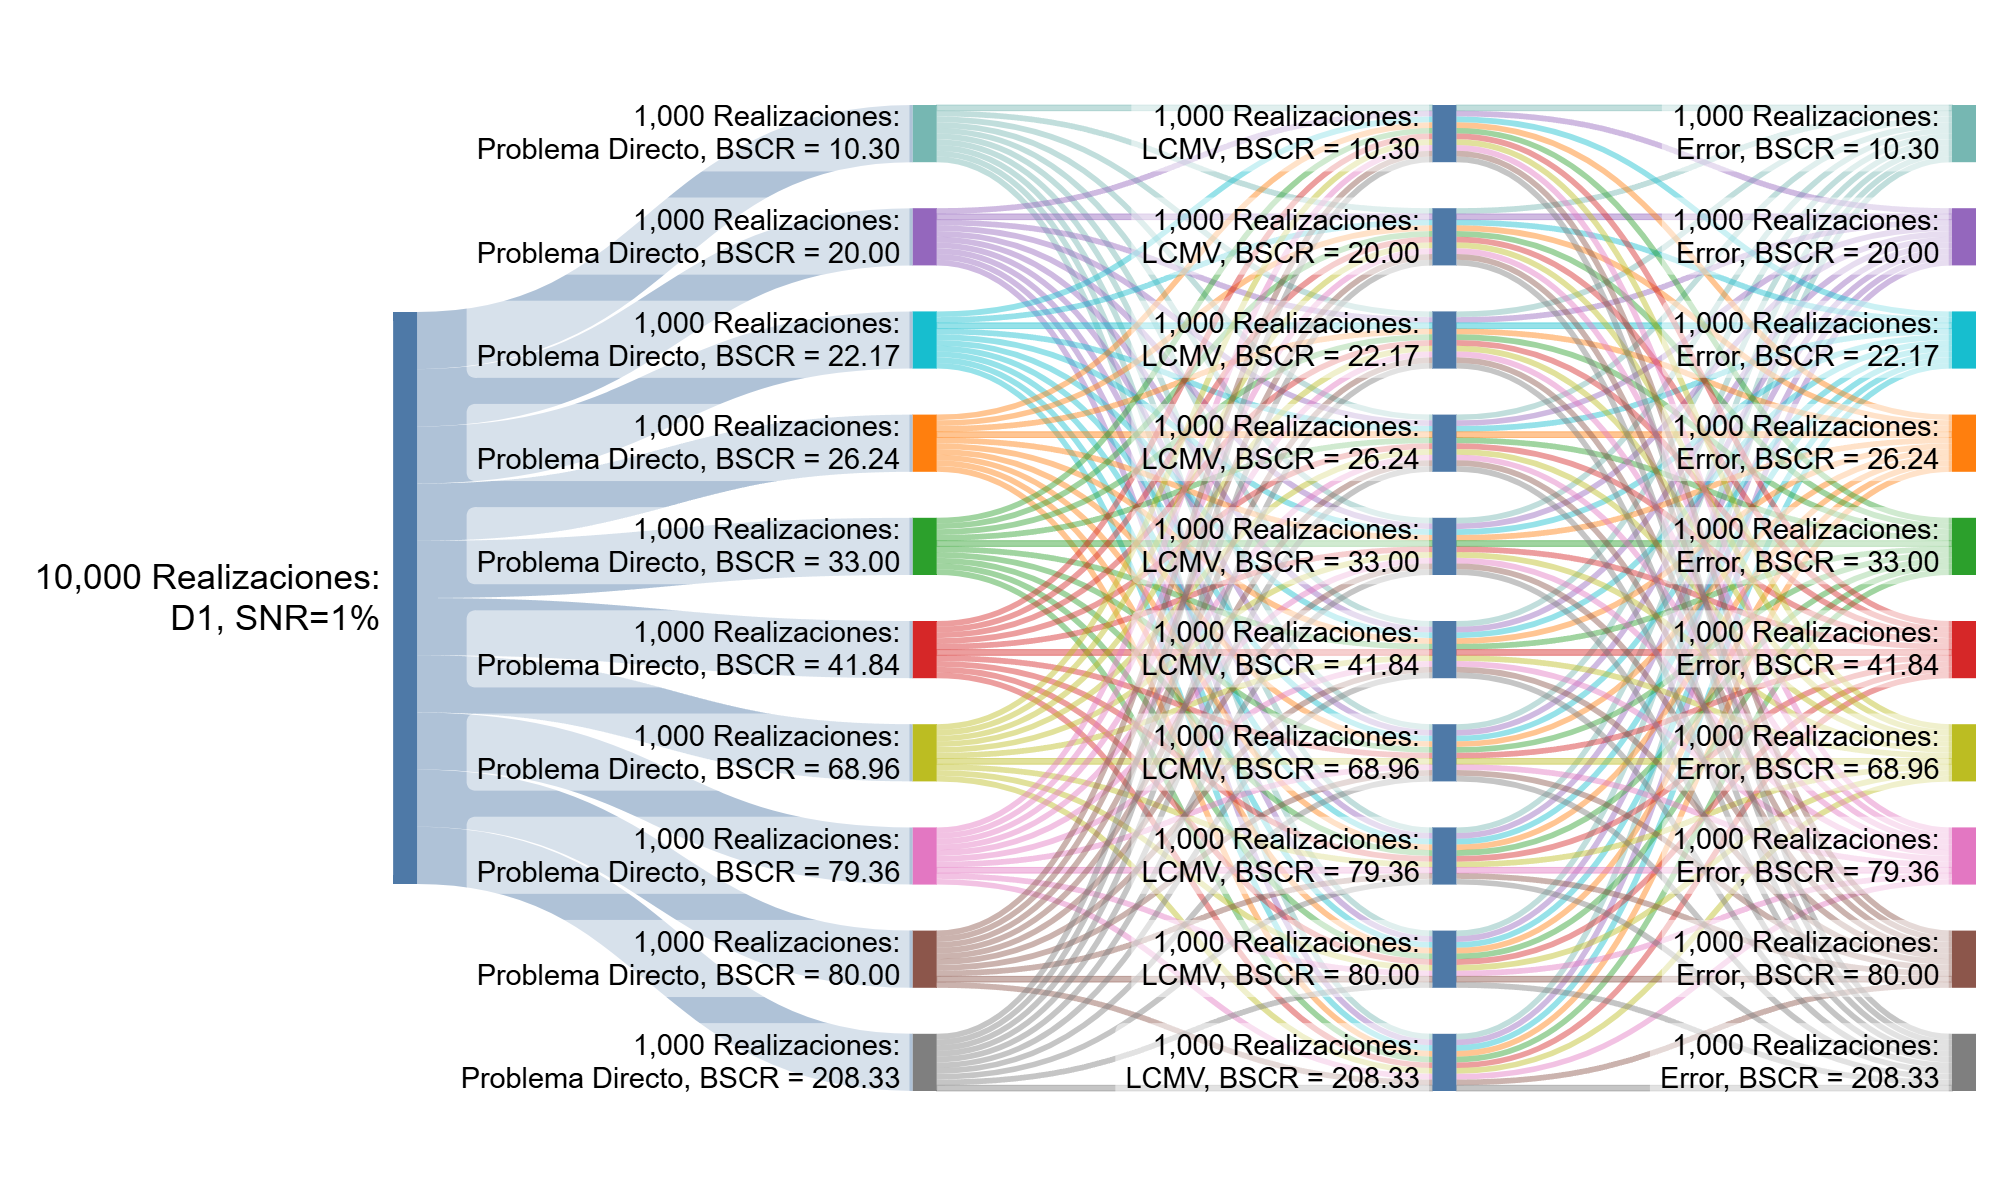
\includegraphics[width=\textwidth]{gfx/sankey-boxplots.png}
    \caption{Diagrama del agrupamiento del error en la localización de la fuente de actividad neuronal sin considerar el valor de BSCR utilizado en la solución del problema inverso. Este describe el caso del dipolo 1 y SNR 1\%, pero se repitió para los dipolos 2 y 3, así como para los niveles de SNR 5\% y 10\%.}
    \label{fig:sankey-boxplots}
\end{figure}

Para visualizar los resultados obtenidos en este agrupamiento, se presentan en la \cref{fig:bscr-performance} los resultados obtenidos en forma de diagramas de caja y bigotes, donde se muestra la distribución de los valores del error en la localización de la fuente de actividad neuronal para cada uno de los BSCR involucrados en el estudio, agrupados por el dipolo y nivel de ruido correspondiente.
Los resultados mostrados corresponden al nivel de SNR = 1\% y 10\% para cada uno de los tres dipolos, ya que estos representan los extremos en la relación señal-ruido y permiten observar el desempeño del error en condiciones de ruido bajo y ruido alto.

Regresando a la \cref{fig:sankey-boxplots}, este diagrama muestra la distribución correspondiente de la \cref{fig:error-overall-d1n1}, donde el nodo del extremo izquierdo representa el espacio de los datos del dipolo 1 con SNR = 1\%, el nodo siguiente representa las simulaciones resultantes del problema directo con todos los valores de BSCR, contiguo a este se encuentran los resultados de la implementación del filtro espacial LCMV en el problema inverso con todos los valores de BSCR, y finalmente, el nodo del extremo derecho representa los resultados obtenidos en la estimación del error en la localización de la fuente de actividad neuronal agrupados por su origen en el problema directo sin considerar el valor de BSCR utilizado en el cálculo del filtro espacial en el problema inverso.
Siendo cada uno de estos últimos nodos, los que se presentan en el eje horizontal de la \cref{fig:error-overall-d1n1}, representando una matriz de forma 1000$\times$10. 

Retomando la \cref{fig:bscr-performance}, cada una de las gráficas nos permite observar y comparar el desempeño del error en la localización de la fuente de actividad neuronal.
En cada gráfica, el eje horizontal muestra los valores de BSCR utilizados en la solución del problema directo, mientras que el eje vertical indica la distribución de los valores del error obtenido en el problema inverso en función de la distancia media entre vértices de la malla de la corteza cerebral.
Las cajas representan el rango intercuartílico de los valores del error, mientras que las líneas horizontales dentro de las cajas representan la mediana de los valores del error, y las muescas cercanas a estas líneas horizontales representan el intervalo de confianza del 95\% de los valores del error
Los bigotes representan el rango de los valores del error, mientras que los puntos fuera de los bigotes representan los valores atípicos de los datos.
Por último, las cruces rojas a los extremos de los bigotes representan los valores extremos de los datos y se encuentran a una distancia de 1.5 veces el rango intercuartílico de los valores del error.
Estos valores extremos se consideran atípicos y aunque pareciera que son numerosos en gráficas como las \cref{fig:error-overall-d2n1,fig:crb-overall-d2n3,fig:error-overall-d3n1,fig:crb-overall-d3n3}, estos representan una fracción mínima de los datos obtenidos, ya que representan cantidades de 20 a 70 valores atípicos de un total de 1000 valores obtenidos en cada permutación.

\begin{figure}[p]
    \centering
    \begin{subfigure}{0.49\textwidth}
        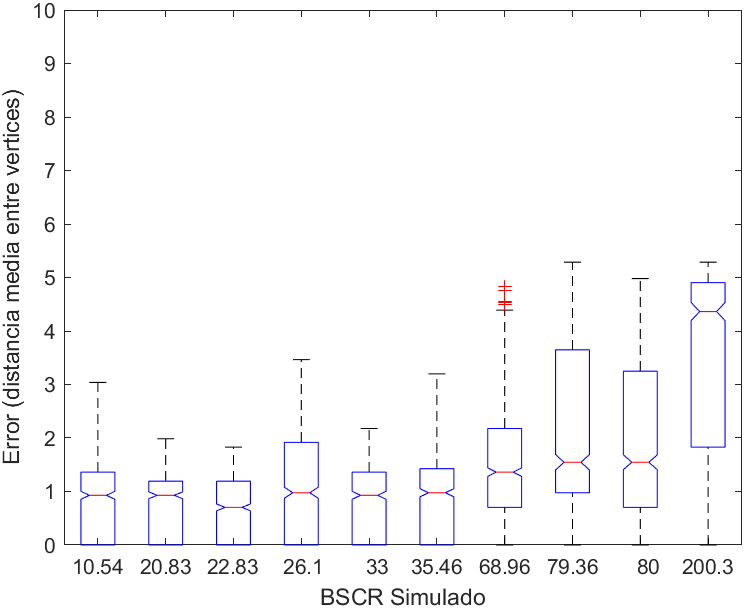
\includegraphics[width=\textwidth]{overall_bscr_error_boxplots_percentile/d1n1.png}
        \caption{Error en la localización de la fuente de actividad neuronal de diferentes BSCR: Dipolo 1, SNR 1\%.}
        \label{fig:error-overall-d1n1}
    \end{subfigure}
    \hfill
    \begin{subfigure}{0.49\textwidth}
        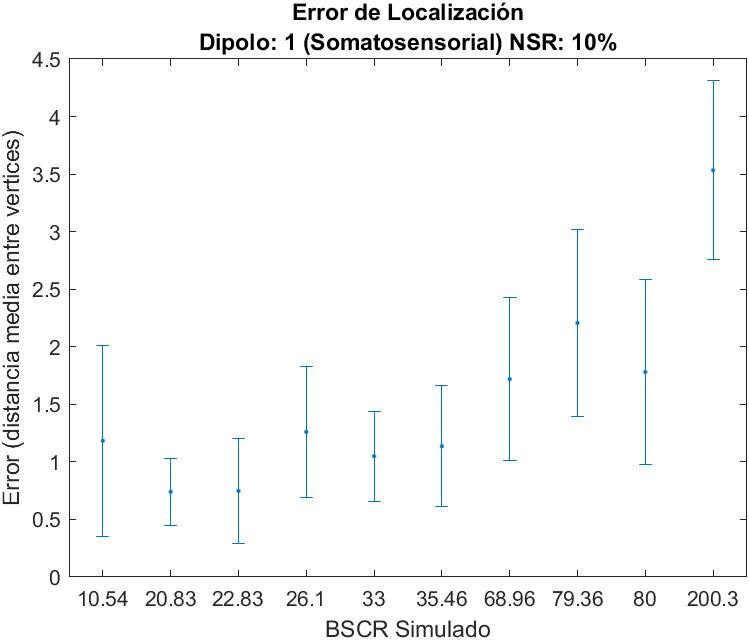
\includegraphics[width=\textwidth]{overall_bscr_error_boxplots_percentile/d1n3.png}
        \caption{Error en la localización de la fuente de actividad neuronal de diferentes BSCR: Dipolo 1, SNR 10\%.}
        \label{fig:crb-overall-d1n3}
    \end{subfigure}
    \vskip\baselineskip
    \begin{subfigure}{0.49\textwidth}
        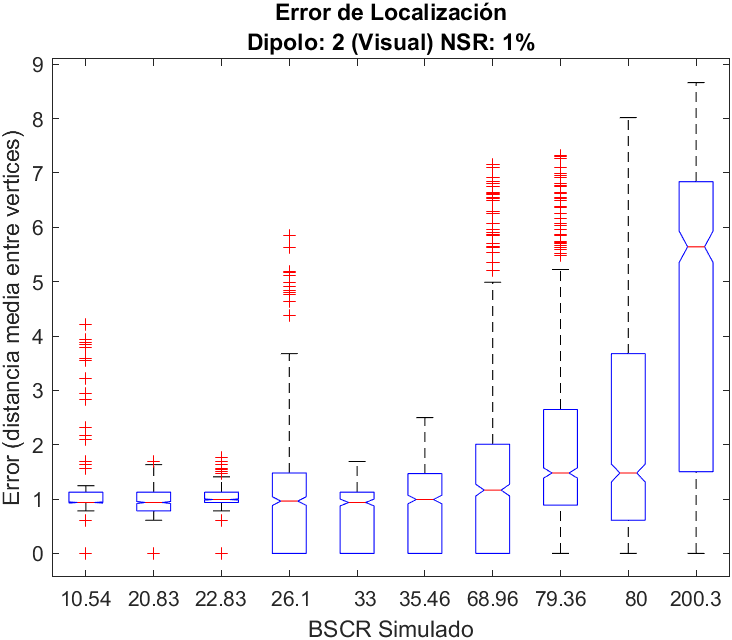
\includegraphics[width=\textwidth]{overall_bscr_error_boxplots_percentile/d2n1.png}
        \caption{Error en la localización de la fuente de actividad neuronal de diferentes BSCR: Dipolo 2, SNR 1\%.}
        \label{fig:error-overall-d2n1}
    \end{subfigure}
    \hfill
    \begin{subfigure}{0.49\textwidth}
        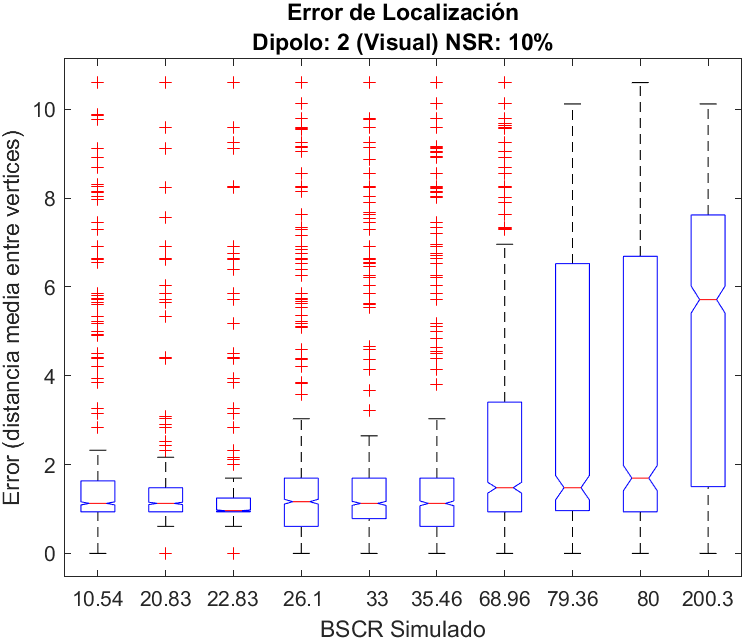
\includegraphics[width=\textwidth]{overall_bscr_error_boxplots_percentile/d2n3.png}
        \caption{Error en la localización de la fuente de actividad neuronal de diferentes BSCR: Dipolo 2, SNR 10\%.}
        \label{fig:crb-overall-d2n3}
    \end{subfigure}
    \vskip\baselineskip
    \begin{subfigure}{0.49\textwidth}
        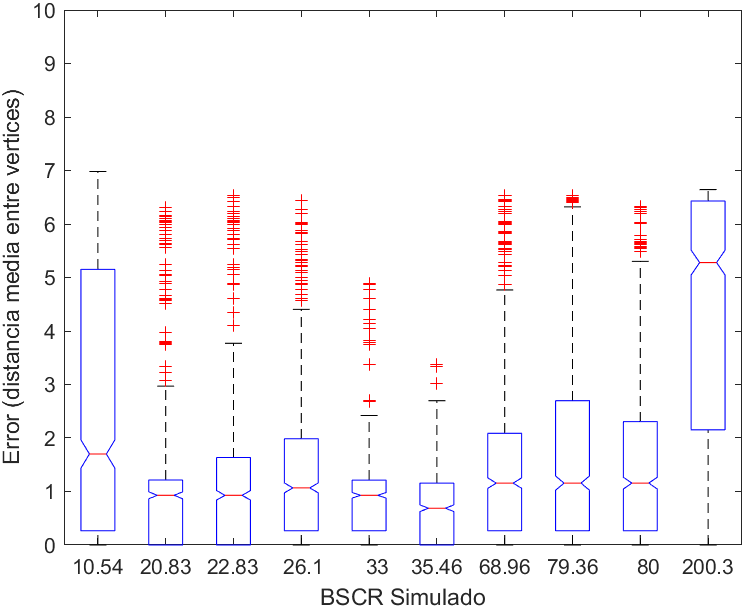
\includegraphics[width=\textwidth]{overall_bscr_error_boxplots_percentile/d3n1.png}
        \caption{Error en la localización de la fuente de actividad neuronal de diferentes BSCR: Dipolo 3, SNR 1\%.}
        \label{fig:error-overall-d3n1}
    \end{subfigure}
    \hfill
    \begin{subfigure}{0.49\textwidth}
        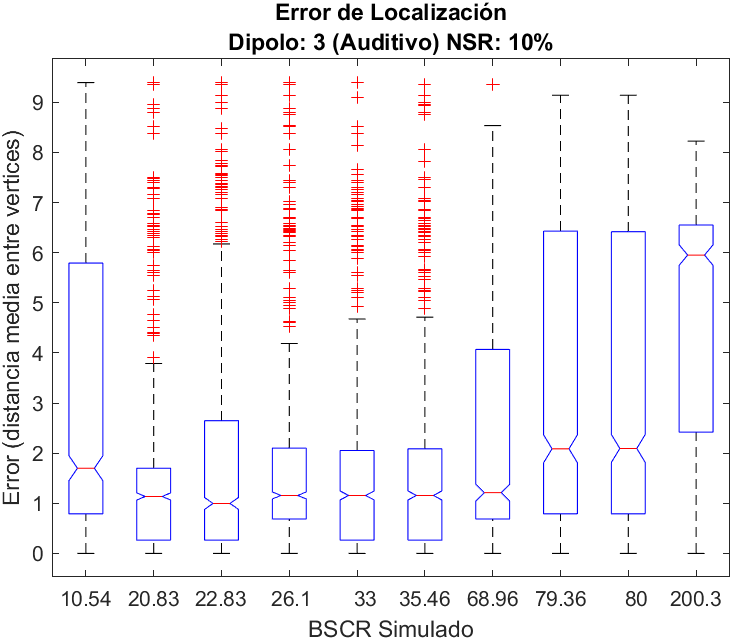
\includegraphics[width=\textwidth]{overall_bscr_error_boxplots_percentile/d3n3.png}
        \caption{Error en la localización de la fuente de actividad neuronal de diferentes BSCR: Dipolo 3, SNR 10\%.}
        \label{fig:crb-overall-d3n3}
    \end{subfigure}
    \caption{Desempeño del uso de diferentes valores de BSCR en la simulación y localización de fuentes de actividad neuronal.}
    \label{fig:bscr-performance}
\end{figure}